\chapter{Related Work}
\label{chapter:relatedwork}
\thispagestyle{myheadings}

\graphicspath{{2_RelatedWork/Figures/}}

\label{sec:history}
\subsection{Resilient Distributed Datasets}
Major methods in Spark are Resilient Distributed Datasets (RDDs), a data structure that abstracts distributed memory across different clusters. 
The immutable coarse-grained transformation, spark-scheduler with lazy-evaluation, and memory management with cacheing achieve computation with fault-tolerance, 
fast execution, and moderate control on memory efficiency \cite{DBLP:conf/nsdi/ZahariaCDDMMFSS12}.

A RDD is essentially a multi-layer Java data structure. A top RDD object references Java array, which intern, references a set of tuple objects. 
The coarse-grained transformations and immutability requires a RDD to be deep-copied to produce a new RDD, but efficiently offers fault tolerance. 
The lost partitions of a RDD can be recomputed in parallel on different nodes rather than rolling back the whole program.

Spark-pipeline consists of sequence of transformations and actions over RDDs. A transformation produces a new RDD from a set of existing RDD. 
An action is method that computes statistics from an RDD. Due to lazy-evaluation nature, transformations do not materialize the newly created RDD. 
Instead, RDD Lineages are created. Lineage is a graph among parent and child RDDs which represents logical execution plan. 
This enhance fault-tolerance and improve ability to optimize execution plan. 

RDDs can be cached in memory for faster access by persist method. Developers can specify a storage level for a persisted RDD, in memory with serialized or deserialized, or on disk. 
Other than persisted RDD, Spark generates a lot of intermediate RDDs during execution. Since RDD is a Java object, they are managed by Garbage Collection (GC) in the JVM. 
However, persisted RDDs are never collected by GC. This GC might cause significant deterioration of performance of Spark, because GC shows heavy overhead when there are a number of objects.


\subsection{Memory Management in Spark}
Spark framework allocates multiple executors, JVMs, that run sequence of transformations and actions. As we describe the previous section, data in Spark is mainly stored as Java objects in memory, 
so that they are allocated on JVM heap and managed by JVM Garbage Collection. The data may form three types \cite{DBLP:journals/pvldb/XuGDWW19}: Cached data, Shuffled data, and Operator-generated data. 

Spark can cache data in memory to reduce disk I/O. This Cached data usually long-lived Java objects and span multiple stages in Spark-pipeline. 
Spark allocates a logical storage space to store the cached data as shown in Figure. After aggregation, Spark generates Shuffled data. Shuffled data is usually long-lived, 
because it need to be kept in memory until the task ends. Spark allocates execution space to store Shuffled data.
The storage space and execution space spans 60 \% of JVM heap space in default. Operator-generated data is data generated by user-defined operations. Since Operator-generated data may or may not be used, 
after the operation finish, the data object can be both short-lived or long-lived objects. These are stored in user space allocated on default 40 \% of JVM heap.

All data of these types on JVM heap is managed by JVM GC. GC check references graph of objects, mark whether the objects are used and deallocate memory space occupied by unused objects. 
There are three popular GCs: Parallel, CMS and G1. All of these method track generation of object based on the region of memory. 
The Java logical heap structure is shown in Figure~\ref{fig:javaheap}. As the figure shows, Java logical heap can be separated into three main parts where store objects for each corresponding generation: 
permanent generation, young generation, and old generation. The region for permanent generation stores metadata required by JVM to describe 
class and method used in application which will be permanently lived on the region of memory. The overview of Java GC is shown in Figure~\ref{fig:javagc}. 
The outer box represents region for particular generation. The inner box and the number represents object and its age in GC. 

The region for young generation mainly consists of two parts: Eden and Survivor space. 
First, Java objects are created in Eden space and promoted to Survivor space when survive from GC. 
After objects survive several GCs in Survivor space, they are finally promoted to old generation.

In region of old generation, JVM lunches multi-thread to perform GC. GC with multi-threading suffers from Stop-The-World (STW) pauses; 
GC may suspend application threads while performing object marking and deallocation. 
Different GC algorithms try to solve this problem with trade-off between GC frequency and memory utilization. 

Because of the problem of STW and copying objects to different physical memory pages , JVM GC cause huge overhead when number of objects is large. 
Therefore, GC become severe issue in Big Data processing where might produce significant number of object.

\begin{figure}[htb]
    \includegraphics[width=15cm]{java_heap.eps}
    \caption{Java Heap Structure}
    \label{fig:javaheap}
\end{figure}

\begin{figure}[htb]
    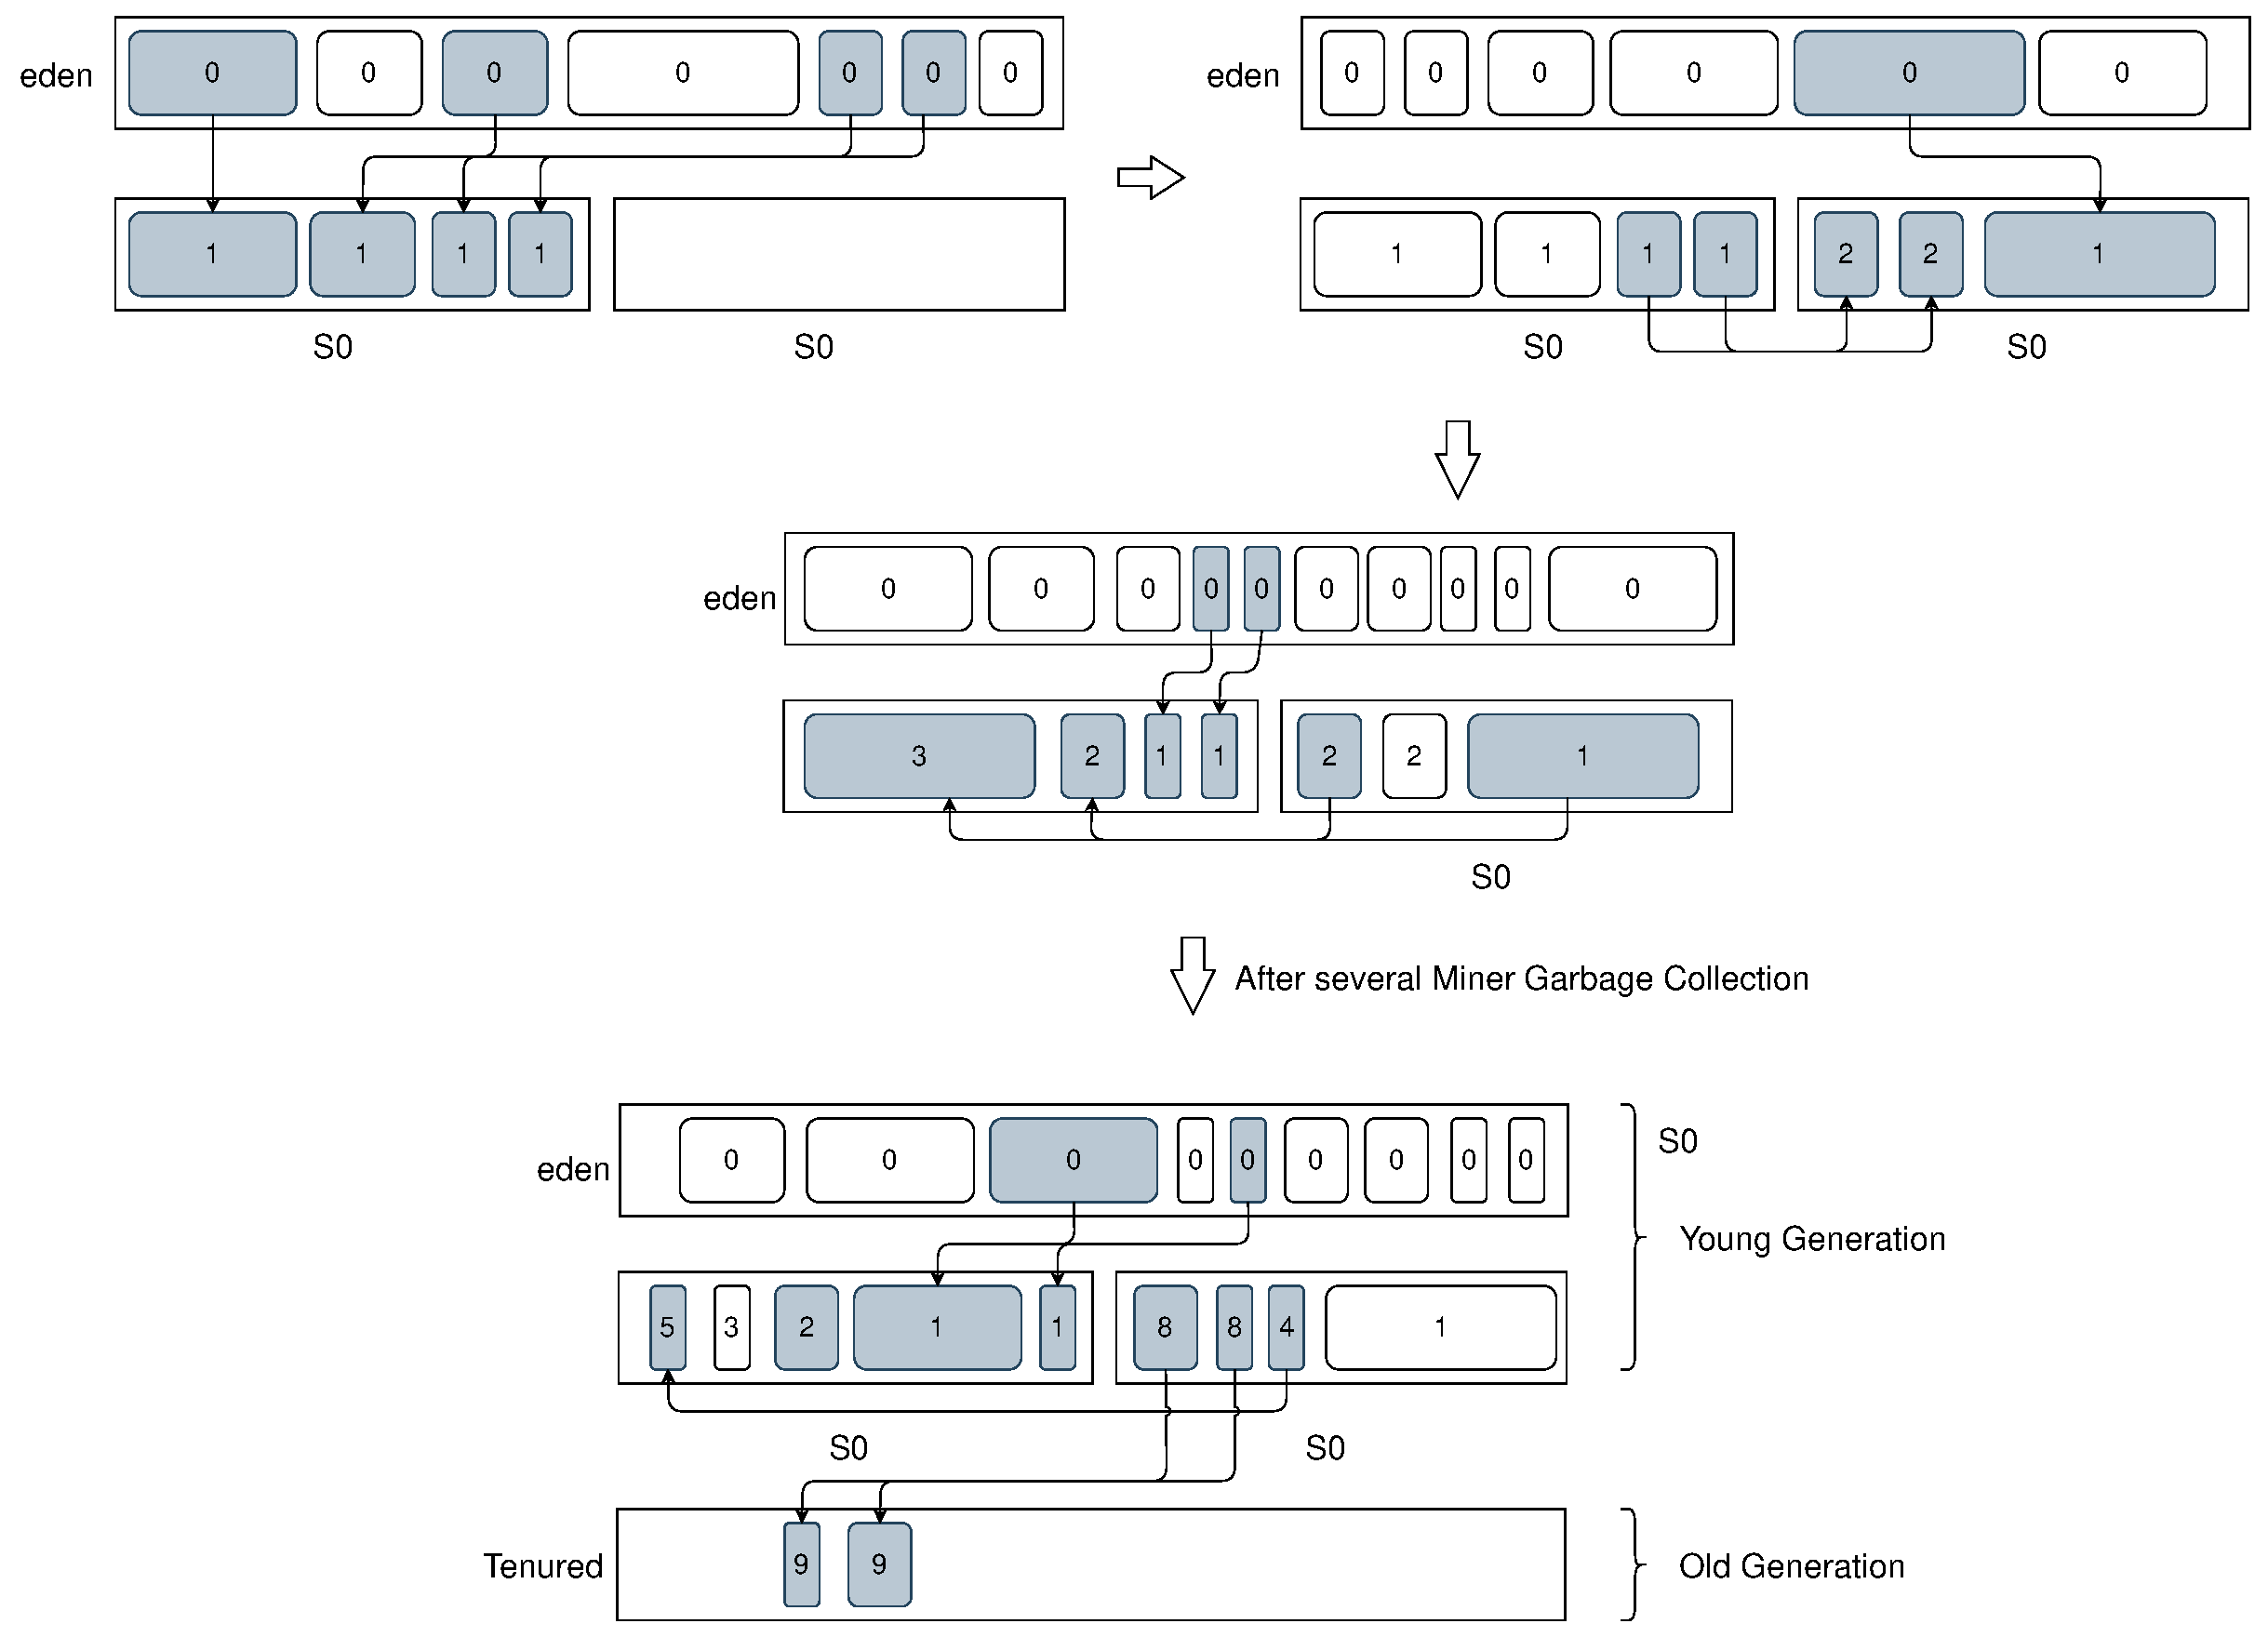
\includegraphics[width=15cm]{java_gc.eps}
    \caption{Java Garbage Collection}
    \label{fig:javagc}
\end{figure}


\subsection{Garbage Collection Tuning}
There are many different ways that one can improve the performance of GC in Java. One of these is for example avoiding pointer-based data structures, such as HashMap and LinkedList. 
These objects have a "wrapper" object for each entry so that number of object tends to be larger than when when an array is used.

Caching serialized object in memory also reduce number of object and memory usage since the set of objects become a byte or binary array. 
Spark SQL applications use DataFrames\cite{DBLP:conf/sigmod/ArmbrustXLHLBMK15}, 
whose intermediate data are managed by an optimized memory manager named Tungsten.
Tungsten stores the intermediate data in a serialized binary form and performs aggregation functions directly on he serialized objects.
Therefore, the number of Java objects in memory is reduced and it reduces the DC frequency and object marking/sweeping. 

In addition, developers can allocate data off-heap of JVM to avoid tracking by GC. 
Facade\cite{DBLP:conf/asplos/NguyenWBFHX15} proposed a compiler and runtime system to bound the number of in-memory data objects, through storing data in an off-heap region and 
manipulating the data with control interfaces.

Although these memory management solution for GC help developer improve performance of Spark applications, 
the effort to discover the best GC tuning afflicts developers.


\clearpage

\section{Serialization}
\label{sec:history}
Paging object solution for faster transportation among clusters
Protocol Buffer 
We cannot serialize pointer (it is difficult to represent complex object in serialized form to interact with).

\clearpage



\section{Elements Copy and Insertion into Size-initialized Vector in Rust.}
\label{sec:history}
In this experiment, four methods are used to insert elements into vector in Rust. One is clone method which performs bitwise deep copy. 
Another is clone\_from which also performs bitwise deep copy, but copies elements of the vector to distination vector rather than 
creating new one. We initialize the distination vector with the same size to the number of elements we insert into it. 
Another is copy\_nonoverlapping function which copies values from source to distination memory region. 
The other is pushing elements of source to distination vector one by one. Insertions of elements with 4 size are conducted 1000000, 1500000, 10000000, 15000000, and, 
their runtimes for each elements type, integer and String are measured. 


The figure shows the result of the experiment. Among the runtime performances of integer insertion for every methods, 
clone, clone\_from, and copy\_nonoverlapping method shows the similar performance. However, the pushing the copy of elements one by one has much slower runtime performance 
compared to the rest. This is because integer elements are allocated contiguously in the memory, so that accessing address of memory by pointer reads some next address. 
This boosts the copy and insertion of elements. 

On the other hand, all of methods show the similar runtime performance in experiment for String object insertion. 
This is because String object is not stored in contiguous memory region. The vector stores pointer to the object and 
process need to access around different memory region again and again to deeply copy the object.

\begin{figure}[htb]
    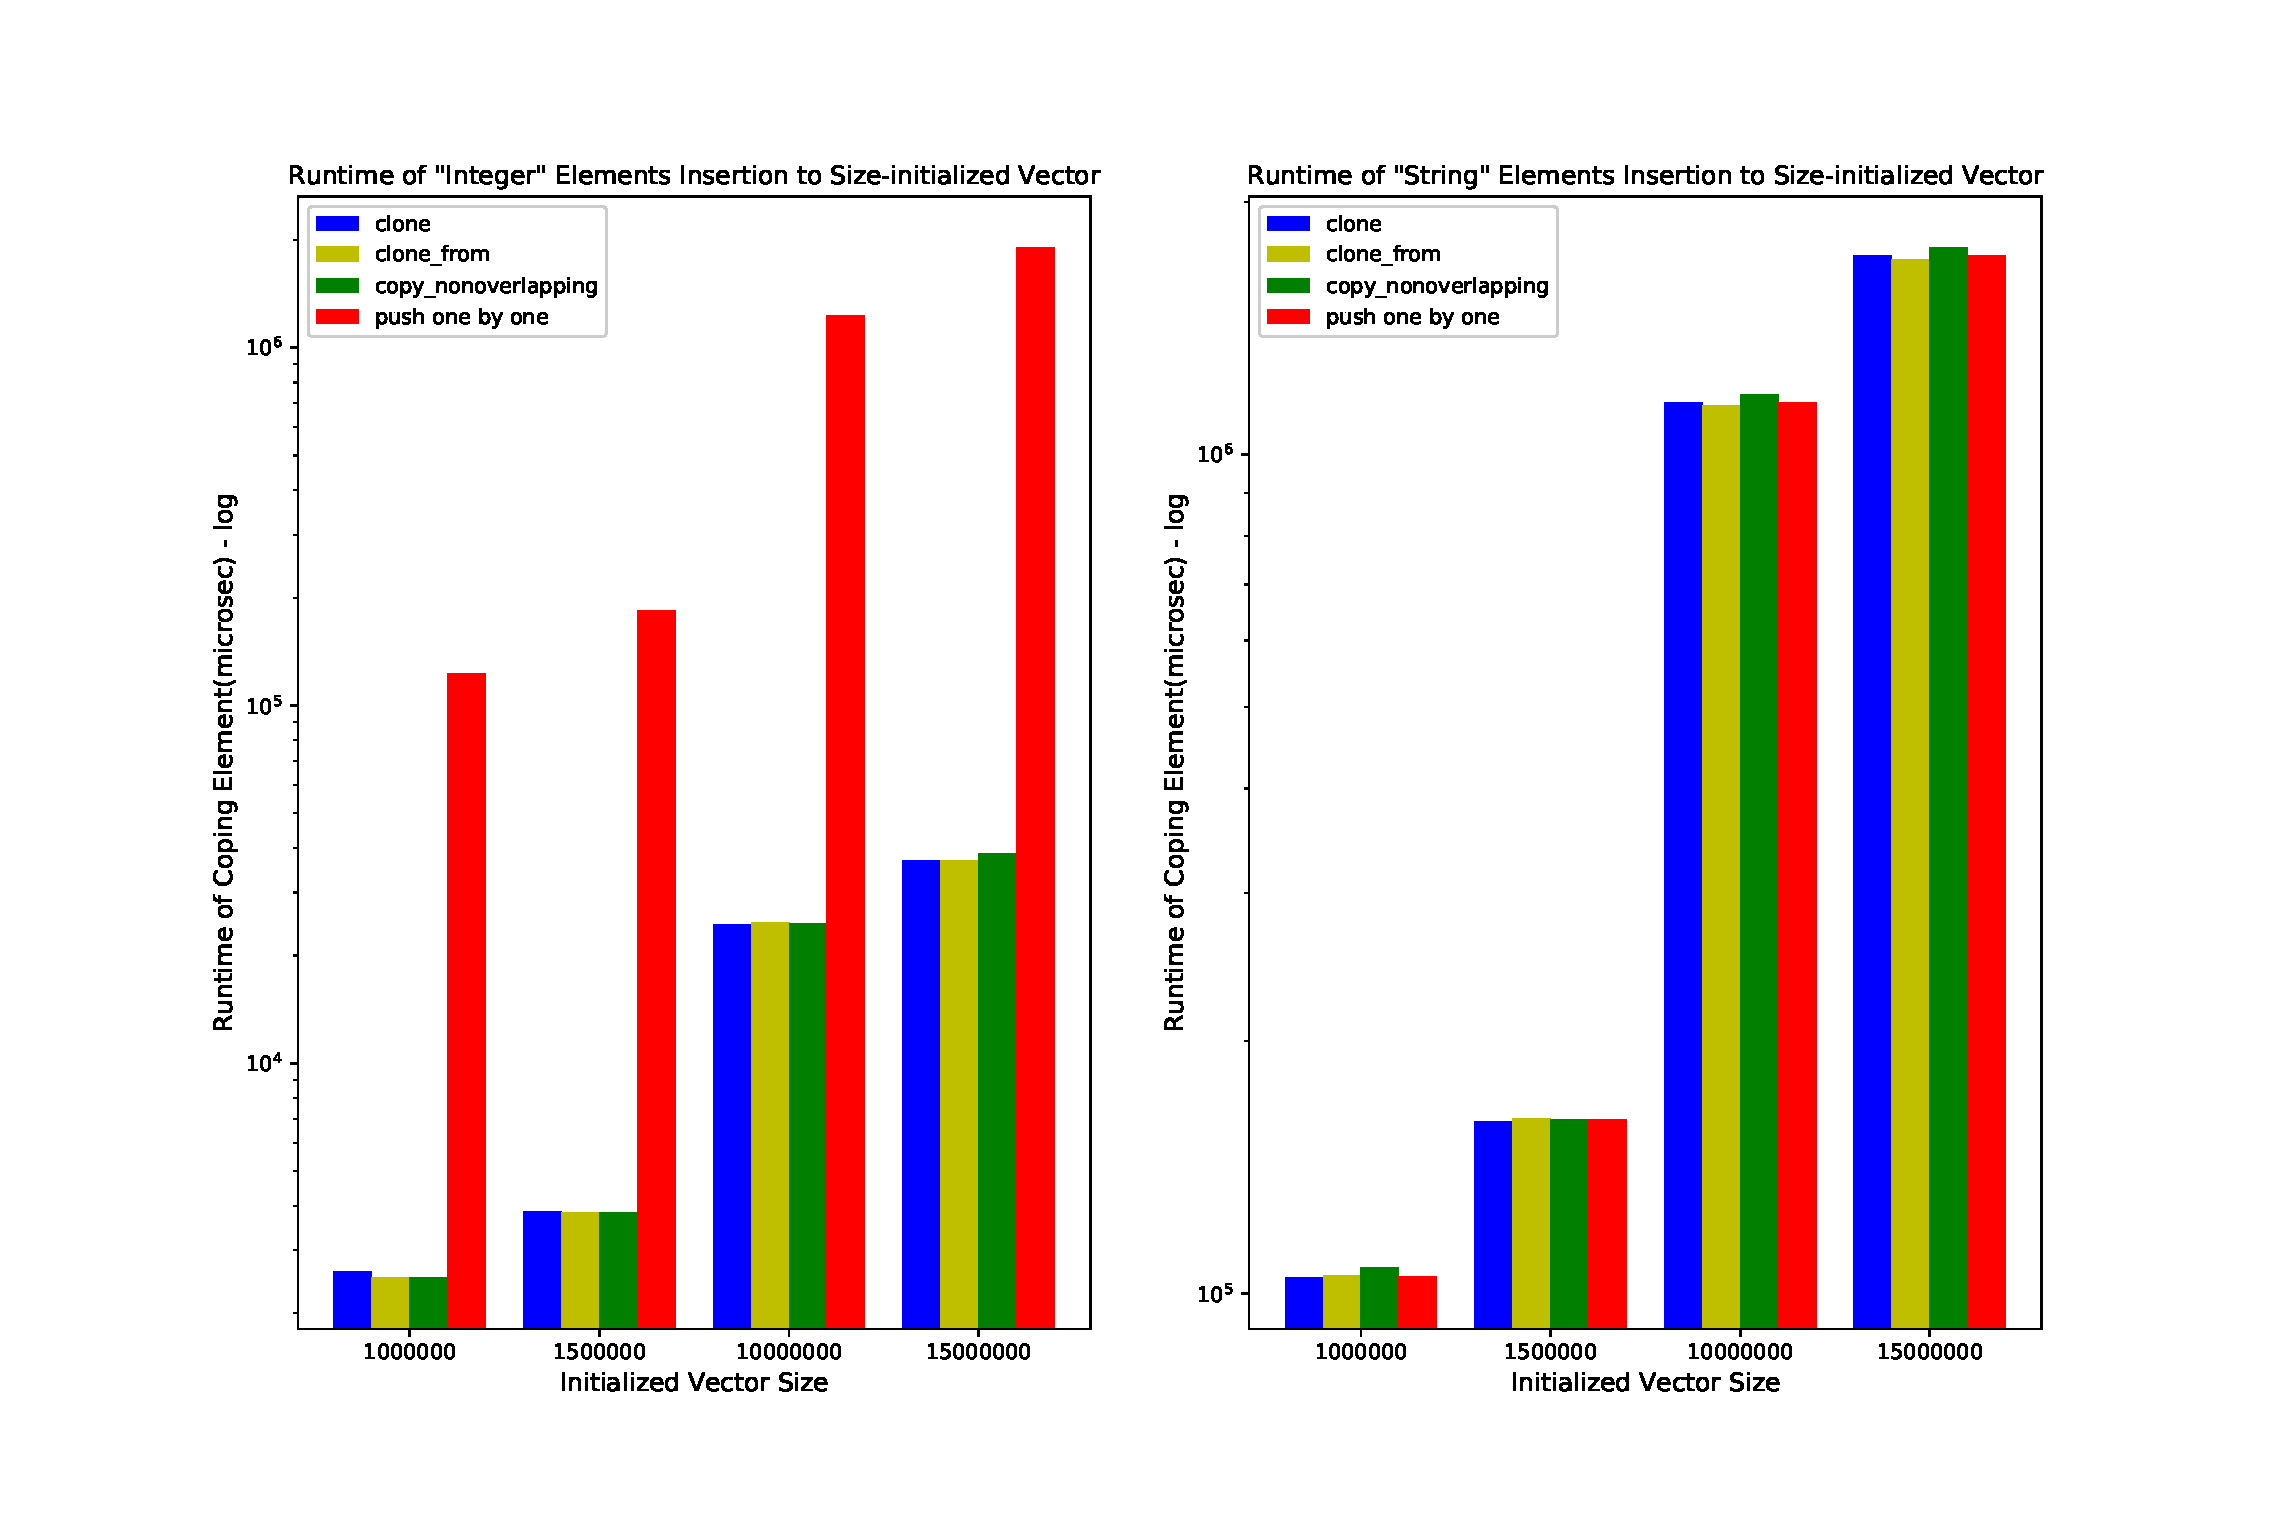
\includegraphics[width=15cm]{rust_various_insertion.eps}
    \caption{Runtime of elements copy from one vector and insertion to the other vector.}
    \label{fig:Sampling}
\end{figure}
\clearpage

\section{Access time to elements in vector}
\label{sec:history}
In this experiment, whether mutability has impacts to operation on the object in terms of runtime performance. 
According to the experiment, there is no difference on accessing to elements of mutable and immutable vector.

\begin{figure}[htb]
    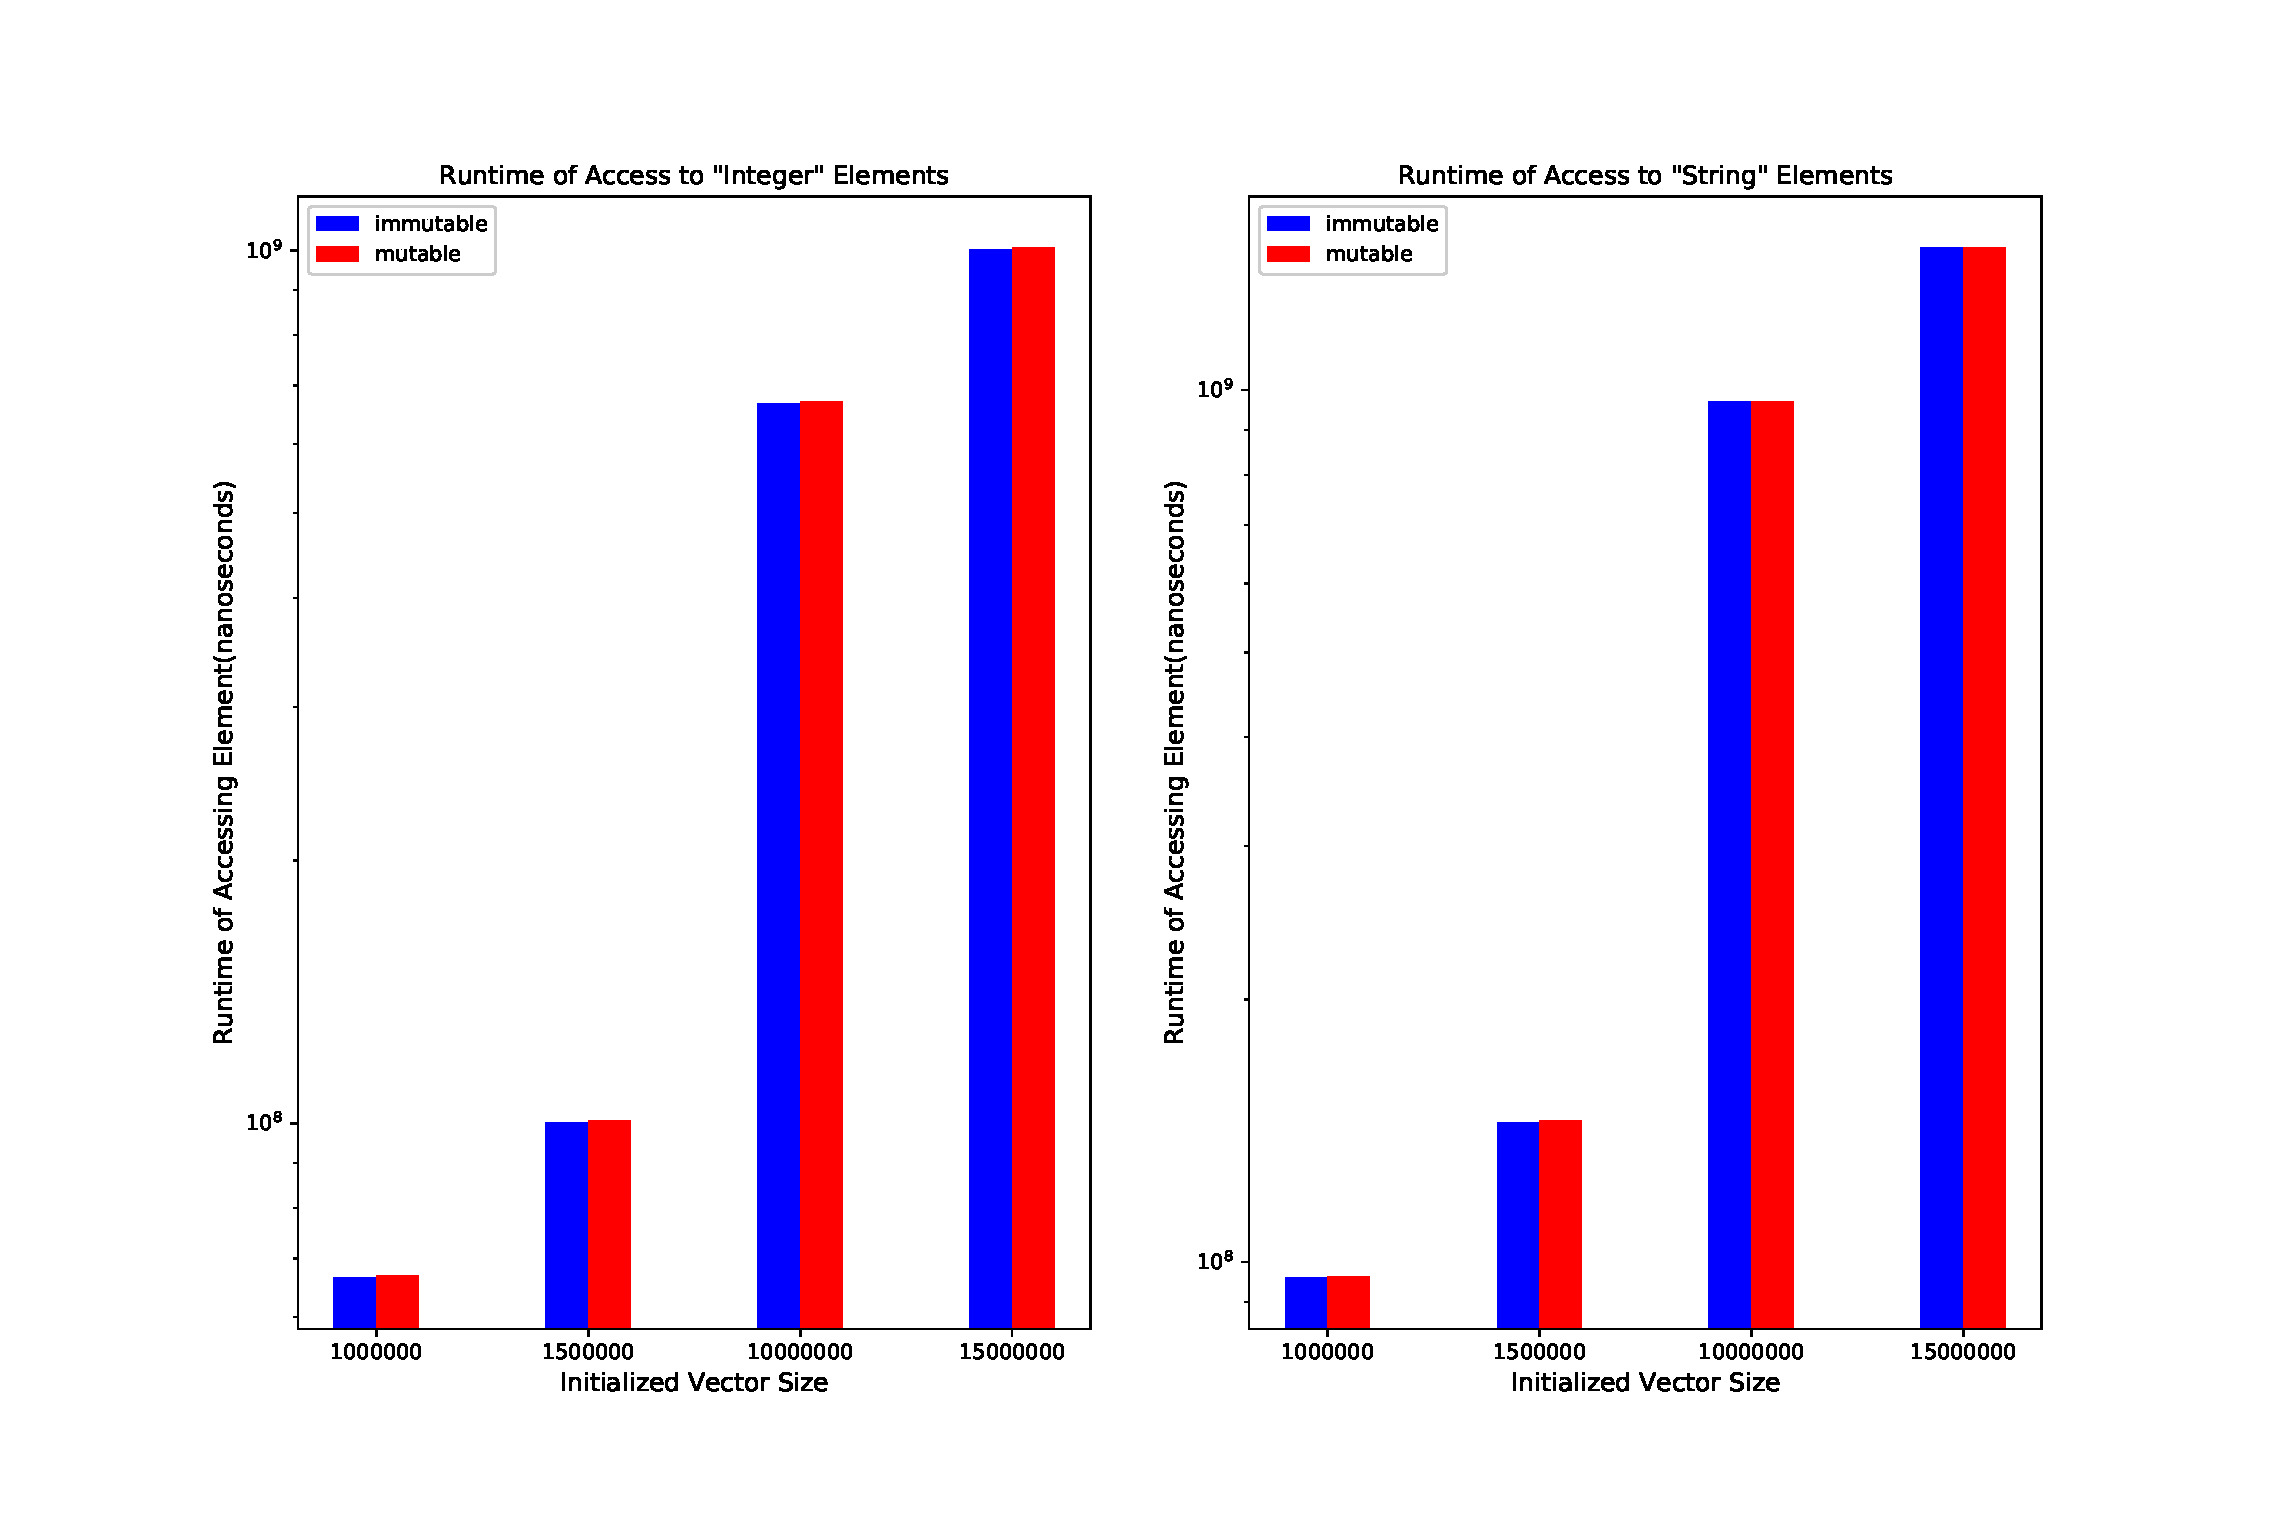
\includegraphics[width=15cm]{rust_various_access.eps}
    \caption{Runtime of elements copy from one vector and insertion to the other vector.}
    \label{fig:Sampling}
\end{figure}

\section{Access time to owned, borrowed, and sliced field of object}
\label{sec:history}
In this experiment, differences of access time to among owned, borrowed, and sliced are observed. 
Each variable has slightly different use of memory. 


\begin{figure}[htb]
    \begin{lstlisting}
        struct CustomerOwned {
            key: i32,
            age: i32,
            num_purchase: i32,
            total_purchase: f64,
            duration_spent: f64, 
            duration_since: f64,
            zip_code: String,
            address: String,
            country: String,
            state: String,
            first_name: String,
            last_name: String,
            province: String,
            comment: String, 
            order: OrderOwned
        }

        struct CustomerBorrowed<'a> {
            key: &'a i32,
            age: &'a i32,
            num_purchase: &'a i32,
            total_purchase: &'a f64,
            duration_spent: &'a f64, 
            duration_since: &'a f64,
            zip_code: &'a String,
            address: &'a String,
            country: &'a String,
            state: &'a String,
            first_name: &'a String,
            last_name: &'a String,
            province: &'a String,
            comment: &'a String, 
            order: &'a OrderBorrowed<'a>
        }

        struct CustomerSlice<'a> {
            key: &'a i32,
            age: &'a i32,
            num_purchase: &'a i32,
            total_purchase: &'a f64,
            duration_spent: &'a f64, 
            duration_since: &'a f64,
            zip_code: &'a str,
            address: &'a str,
            country: &'a str, 
            state: &'a str,
            first_name: &'a str,
            last_name: &'a str,
            province: &'a str,
            comment: &'a str,
            order: &'a OrderSlice<'a>
        }

        struct CustomerRc {
            key: Rc<i32>,
            age: Rc<i32>,
            num_purchase: Rc<i32>,
            total_purchase: Rc<f64>,
            duration_spent: Rc<f64>, 
            duration_since: Rc<f64>,
            zip_code: Rc<String>,
            address: Rc<String>,
            country: Rc<String>,
            state: Rc<String>,
            first_name: Rc<String>,
            last_name: Rc<String>,
            province: Rc<String>,
            comment: Rc<String>, 
            order: Rc<OrderRc>
        }
    \end{lstlisting}
    \caption{Representation of Customer object in Rust.}
    \label{fig:Sampling}
\end{figure}

\clearpage



\section{Possible Graph Structure in Rust}
\label{sec:history}
In Rust, there are two essential problems to construct graph structure, lifetime and mutability. 

The first problem is about what kind of pointer to use to point to other nodes. 
Since graph can be cyclic, so the ownership consept in Rust is violated if we use Box$<$Node$>$.

All of graph structure are immutable at least at creation time. Because graph may have cyclic, 
we can not create graph at one statement. Although edge of graph has to be mutable to create entire graph structure, 
we might need multiple references to edges, which violates basic rule of Rust programming.

One solution is to use raw pointers. This is the most flexible approach, but also the most dangerous. 
By taking this way, we are ignoring all the benefits of Rust.

\section{Experiment for Multithread}
\label{sec:history}
Experiment for multithreading in Rust is interesting, because there are many memory allocation and deallocation in each threads.
This is because each thread offten need to form independent memory state to each other to perform computation concurrently safely.
In addition, the multithreading strategy can be planned in different ways in Rust using different concurrent computation tools, 
Mutex, Arc, spawn, channel, scope, and so on.

Currently available plan
\begin{itemize}
    \item spawn, channel and sending data (currently deviding data, but we probably do not need to).
    \item spawn, forkjoin and shared data.(shared data among child and parent).
    \item scope, forkjoin and slice shared data.
    \item Use linkedList instead of Vector (Each node can be sharable data structure). When we have complex object of elements in vector, we want to copy the pointer to the object.
    \item Compare performace on LinkedList which is not contiguous allocation, but do not need additional memory allocation and Vec.
\end{itemize}



\section{Note for next}
\label{sec:history}
Complex object of elements copy and insertion among vector is worth to experiment. This can be compared with Java,
because memory layouts of struct in Rust and class in Java are different. Rust stores fieds in the contiguous memory region. 
However, Java stores field elements to different region.

Complex object whose fields has reference elemenets insertion to vector can be evaluated. Operation to the fields can be little 
more expensive because the pointer to the value of the field is not stored in contiguous memory region.

Generic type and static type function can be compared. 

To optimise access to String elements of vector, smallstring can be improve the runtime performance. 
This is because the smallstring optimization enables short length of string on stack as byte array. 
This string type sets condition where it makes decition where the string is stored on heap or stack as array at certain length.

Comparing operation on reference and owned variable is also interested to examine.

Comparing operation on various smart pointer type. 
Rc$<$T$>$ enables value to have multiple owners, but the value should be immutable. Rc$<$T$>$ is used in case of single thread. 
When the situation is multi-thread, Arc$<$T$>$ is used. Arc$<$T$>$ performs atomic operation, so it is more expensive than Rc$<$T$>$. 
When we need to mutate value of Rc$<$T$>$, RefCell$<$T$>$ can be useful. RefCell$<$T$>$ allow us to have mutiple mutable reference and immutable
of reference mutable or immutable variable at the same time. When the mutability consistency is voilented, it terminates program during runtime. 
That is why RefCell$<$T$>$ is expensive so that the state of mutable consistency should tracked. 
As Cell$<$T$>$, the value is copied in and out of the Cell$<$T$>$ instead of getting refrence to it. 
In addition, Mutex$<$T$>$ provides intetior mutability across multi-thread.

Comparison between mutable and immutable tree or graph structure can be checked. 
This is because tree structure requires Rc$<$T$>$ or Week$<$T$>$ and in addition RefCell$<$T$>$ to make it mutable.

Design experiment for Trait object and Generic function. 
We can have Trait object which is pointer to object which imprements its Trait and use the method of Trait object.
This object has additional information other than just reference to tye original object. 
This is because Rust needs the type information to dynamically calll the right method of Trait object depending on the type of 
original object.
On the other hand, we can have Generic function whose parameter types are Generic types corresponding to Trait. 
When Rust compiles the code, it emits independent function corresponding to every types that implements the Trains specified in parameter.

Vector of Trait object (need to put element into Box) vs Vector of concrete type.


If we keep first created owner until the last phase, we can use borrowing to operate.
If we delete first created owner during the operation, we should use Rc$<$T$>$.
The question would be, we can use Rc$<$T$>$ every where?

Multithread in Rust vs Java

Smart pointer
\begin{itemize}
    \item Box$<$T$>$: Box pointer lets value allocated on heap rather than on the stack.
    \item Rc$<$T$>$: Reference counted pointer lets variable take multiple immutable ownership.
\end{itemize}

Interier mutability
\begin{itemize}
    \item Cell$<$T$>$: For only Copy type, it allows us to mutate variable, even if it is immutable. Howeever, it does not support sharing the variable so that it returns always copy of the value.
    \item RefCell$<$T$>$: This support sharing and interier immutability for all types. This is done by allowing to get mutable reference from immutable variable and push the error detacting time from compile time to runtime.
\end{itemize}    

\section{LLVM}
\label{sec:history}
LLVM (Low Level Virtual Machine) is an umbrella project which contains components of compilation of programming language.
Exsiting compilers have tightly coupled functionalities so that it is not possible to embed them into other applications.
However, the abstract framework of LLVM decouples the functionalities into peaces and the peaces of functionalities can be reused.

In structure of a compiler, there are three main components; flontend, optimizer, and backend. 
In flontend, a develper designs the interface of source programming language in way where it can be optimized by optimizer. 
Then, backend takes optimized code and produce the native machine code. LLVM has a component called LLVM Intermediate Representation (IR), 
which places itself across frontend to optimizer. IR is designed to host mid-level analyses and transformations that you find in optimizer section of a compiler.
High-level language has many common structures and functionalities, so most of all high-level program languages can be represented with IR. 
Once source code is represented with IR, optimizer can easily find pattern and optimize it in faster time. 
IR is useful in terms of flontend. This is because developer of language flontend need to know only how the IR works and use the framework to develop a language.

\section{The existing Big Data tools}
\label{sec:history}
The existing Big Data tools are JVM based. JVM abstract hardware so that JVM can rarely achieve near-native speed. A garbage collector is a

\section{Experiment: Tree aggregate}
\label{sec:history}
Three aggregate can be more memory de/allocation intensive experiment, when we load data from disk line by line to aggregate.
This is because, we will allocate many small objects and deallocate them many times.
We can imitate ShuffledRDDs by writing result to disk and reading it to other thread.  
We can compare to Java implementation for ration of runtime increase.





\section{Todos}
\label{sec:history}
\begin{itemize}
    \item 
    \item Redo the experiment with appropriate size
    \item Document for Memory Management of Java with Garbage Collection and the impact for Big Data tools
    \item The safety of Region Based Memory Management and advantage of using Rust.
    \item Serialize problem 
    \item Document for reference counting(measure dropt time using criterion)
    \item Design experiment for Graph
    \item Design experiment for Multithread
    \item Study about LLVM
    \item Buffer pool
\end{itemize}

\section{Done}
\label{sec:history}
\begin{itemize}
    \item Study about OS memory management
\end{itemize}


\section{Time Line}
\label{sec:history}
\begin{itemize}
    \item End Feb: Finish Experiment for Multithread and Graph
    \item Mid May: ML experiment
    \item End May: Redo experiment with bench mark dataset.
    \item Start April: Finish Writing for first revise.
\end{itemize}


